\documentclass{unitothesis}

% \includeonly{Files/Part1/layer}

% Packages for TikZ NNs
\usepackage{listofitems} % for \readlist to create arrays
\usetikzlibrary{arrows.meta} % for arrow size
\usepackage[outline]{contour} % glow around text
\contourlength{1.4pt}

% COLORS for TikZ NNs
\colorlet{myred}{red!80!black}
\colorlet{myblue}{blue!80!black}
\colorlet{mygreen}{green!60!black}
\colorlet{myorange}{orange!70!red!60!black}
\colorlet{mydarkred}{red!30!black}
\colorlet{mydarkblue}{blue!40!black}
\colorlet{mydarkgreen}{green!30!black}

% STYLES for TikZ NNs
\tikzset{
    >=latex, % for default LaTeX arrow head
    node/.style={thick,circle,draw=myblue,minimum size=22,inner sep=0.5,outer sep=0.6},
    node bias/.style={node,black!90,draw=black,fill=black!25},
    node in/.style={node,green!20!black,draw=mygreen!30!black,fill=mygreen!25},
    node hidden/.style={node,blue!20!black,draw=myblue!30!black,fill=myblue!20},
    node out/.style={node,red!20!black,draw=myred!30!black,fill=myred!20},
    connect/.style={thick,mydarkblue}, %,line cap=round
    connect arrow/.style={-{Latex[length=4,width=3.5]},thick,mydarkblue,shorten <=0.5,shorten >=1},
    node 0/.style={node bias}, % node styles, numbered for easy mapping with \nstyle
    node 1/.style={node in},
    node 2/.style={node hidden},
    node 3/.style={node out}
}
\def\nstyle{int(\curr<\Nnodlen?min(2,\curr):3)} % map layer number onto 1, 2, or 3

% Reset section counter after new part
\usepackage{chngcntr}
\counterwithin*{section}{part}

% Useful commands for this project
\newcommand{\J}{\mathcal{J}}
\newcommand{\mono}[1]{\texttt{#1}}
\newcommand{\mfnet}{\mono{mfnet}\xspace}
\newcommand{\shape}[2]{$#1\times #2$}
\newcommand{\wrt}{with respect to\xspace}
\newcommand{\nin}{n_\text{in}}
\newcommand{\nout}{n_\text{out}}

% Acronyms
\acrodef{FFCNN}{Feedforward Fully Connected Neural Network}
\acrodef{MSE}{Mean Squared Error}
\acrodef{CE}{Cross Entropy}
\acrodef{NN}{Neural Network}
\acrodef{GD}{Gradient Descent}
\acrodef{SGD}{Stochastic Gradient Descent}

% \usepackage{subcaption}

% \usepackage{listings}

% \definecolor{Blue}{rgb}{0.2,0.2,0.9}
% \definecolor{Green}{rgb}{0,0.6,0}
% \definecolor{Gray}{rgb}{0.5,0.5,0.5}
% \definecolor{Purple}{rgb}{0.58,0,0.82}
% \definecolor{background}{rgb}{0.98,0.98,0.95}

% \lstdefinestyle{mystyle}{
%     backgroundcolor=\color{background},
%     commentstyle=\color{Green},
%     keywordstyle=\color{Blue},
%     numberstyle=\tiny\color{Gray},
%     stringstyle=\color{Purple},
%     basicstyle=\ttfamily\footnotesize,
%     basewidth=5.2pt,
%     breakatwhitespace=false,
%     extendedchars=true,
%     breaklines=true,
%     captionpos=b,
%     keepspaces=true,
%     numbers=left,
%     numbersep=5pt,
%     showspaces=false,
%     showstringspaces=false,
%     showtabs=false,
%     tabsize=4
% }
% \lstset{style=mystyle}

% \newcommand{\up}[1]{\uparrow_{\vu{#1}}}
% \newcommand{\down}[1]{\downarrow_{\vu{#1}}}
% \renewcommand{\dag}[1]{#1^\dagger}

\author{Francesco Marchisotti}
\title{\centering\mfnet \sc-- A simple\\[0.5em] Machine Learning Library}
\aayear{2024/2025}

\begin{supervisors}
   \supervisor{}{}{\sc Matteo Osella}
\end{supervisors}

\begin{document}

\maketitlepage
\thispagestyle{empty}
\subsection*{\centering Abstract}
This document presents \mfnet, a simple machine learning library developed as a final project for the \href{https://fisica-sc.campusnet.unito.it/do/storicocorsi.pl/Show?_id=curx_2324}{Deep Learning course}. The key feature is the implementation of the backpropagation algorithm, enabling the training of \aclp*{NN} through gradient descent.

The library is then compared with PyTorch on two simple tasks: a regression (on the California Housing dataset) and a classification (on the MNIST dataset).
\newpage

{\hypersetup{linkcolor=black}\tableofcontents}
% \newpage

\addcontentsline{toc}{section}{Signal Flow in \aclp*{NN}}
\section*{Signal Flow in \aclp*{NN}}

A \ac{FFCNN} is a \ac{NN} architecture where each neuron in one layer is connected to every neuron in the subsequent layer.

\begin{figure}[h]
    \centering
    % NEURAL NETWORK with coefficients, arrows
    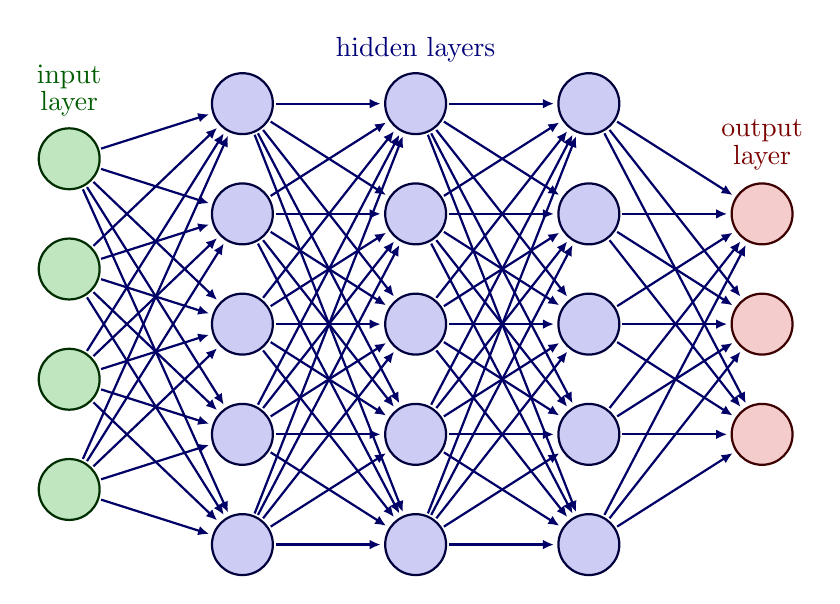
\begin{tikzpicture}[x=2.2cm,y=1.4cm]
    \readlist\Nnod{4,5,5,5,3} % array of number of nodes per layer

    \foreachitem \N \in \Nnod{ % loop over layers
        \edef\curr{\Ncnt} % alias of index of current layer
        \pgfmathsetmacro\prev{int(\Ncnt-1)} % number of previous layer
        \foreach \i [evaluate={\y=\N/2-\i; \x=\curr; \n=\nstyle;}] in {1,...,\N}{ % loop over nodes

        % NODES
        \node[node \n] (N\curr-\i) at (\x,\y) {};

        % CONNECTIONS
        \ifnum\curr>1 % connect to previous layer
            \foreach \j in {1,...,\Nnod[\prev]}{ % loop over nodes in previous layer
                \draw[connect arrow] (N\prev-\j) -- (N\curr-\i); % connect arrows directly
            }
        \fi

        }

    }

    % LABELS
    \node[above=0.3,align=center,mygreen!60!black] at (N1-1.90) {input\\[-0.2em]layer};
    \node[above=0.1,align=center,myblue!60!black] at (N3-1.90) {hidden layers};
    \node[above=0.8,align=center,myred!60!black] at (N\Nnodlen-1.90) {output\\[-0.2em]layer};

    \end{tikzpicture}
    \caption{\Iac{FFCNN}.}
    \label{fig:fcnn}
\end{figure}

A \ac{FFCNN} learns by iteratively performing two main steps: the forward pass and the backward pass.

\paragraph{Forward pass} The input data is propagated through the network, layer by layer, to produce an output prediction. This prediction is then compared to the true target values using a loss function, which quantifies the prediction error.

\paragraph{Backward pass} The network uses the computed loss to adjust its internal parameters. This is done by propagating the error backward through the network and updating the weights to minimize the loss. The process of forward and backward passes is repeated for multiple iterations, gradually improving the model's performance.

This step is the heart of the learning process, as it allows the network to learn from its mistakes and improve its predictions over time.


\section{Basic Data Structure} \label{sec:tensor}

The fundamental data structure in \mfnet is the tensor. In this context, a tensor is simply a \mono{numpy} array with a fixed data type of \mono{numpy.float64}. 

Tensors are used throughout \mfnet to represent inputs, outputs, intermediate activations, weights, and gradients within the \acl{NN}.

\paragraph{Conventions and shapes} Throughout \mfnet:
\begin{itemize}
    \item columns are samples and rows are features/channels;
    \item tensors are bias-augmented unless stated otherwise: the first row is a constant row of ones that propagates through Linear layers (see \cref{sec:layer}). Activation layers copy this row unchanged, and losses temporarily remove it before computing metrics (see \cref{sec:loss}).
\end{itemize}

Canonical shapes (with $m$ being the mini-batch size or the dataset size depending on context):
\begin{itemize}
    \item inputs $X \in \mathbb{R}^{(n_\text{features}+1)\times m}$ after bias augmentation;
    \item linear weights $W^{[l]} \in \mathbb{R}^{(\nout+1)\times(\nin+1)}$ with the first row fixed to $\mqty(1 & 0 \cdots 0)$ (non-learnable);
    \item pre-activations and activations $Z^{[l]}, A^{[l]} \in \mathbb{R}^{(\nout+1)\times m}$ (see \cref{sec:backprop,sec:layer});
    \item targets:
    \begin{itemize}
        \item regression: $Y \in \mathbb{R}^{n_\text{targets}\times m}$ (the loss removes/ignores any bias row if present);
        \item classification: one-hot $Y \in \mathbb{R}^{C\times m}$ with $C$ classes; the loss operates on logits with the bias row removed and restores a zero row in the gradient.
    \end{itemize}
\end{itemize}

\textbf{Important note:} These conventions apply only to the internal workings of \mfnet. There might be some functions that violate these conventions; every function is thoroughly documented and clearly states the shape of the input it is designed to work with. End users are expected to provide the data in standard \shape{m}{\nin} and \shape{m}{n_\text{targets}} or \shape{m}{C} matrices, and \mfnet handles the translation via the \mono{DataLoader} class (see \cref{sec:dataloader}).

\section{Backpropagation} \label{sec:backprop}
Before diving into the details of the implementation of \mfnet, it's necessary to understand the algorithm at the core of the learning process: backpropagation. The goal of the backpropagation algorithm is to compute the derivative of the loss \wrt each weight in the network using the chain rule. The algorithm is more easily understandable using the index notation, but in order to implement it in code, we need to express it in matrix form, so both formulations will be shown.


\subsection{Index notation} \label{sec:index_notation}
We start by defining the following quantities:
\begin{itemize}
    \item $L$: the total number of layers in the network;
    \item $n^{[l]}$: the number of neurons in layer $l$ (with $l = 1$ being the input layer, and $l = L$ being the output layer);
    \item $z_j^{[l]}$: the pre-activation of neuron $j$ in layer $l$. This is the output of the linear transformation in layer $l$ and the input of the activation function;
    \item $a_j^{[l]}$: the activation of neuron $j$ in layer $l$ (with $a_j^{[0]} = x_j$, and $a_j^{[L]} = \hat{y}_j$). This is the output of layer $l$ and the input of layer $l+1$;
    \item $W_{jk}^{[l]}$: the weight connecting neuron $k$ in layer $l-1$ to neuron $j$ in layer $l$ (with $W_{j1}^{[l]} = b_j^{[l]}$);
    \item $g$: the activation function used in the hidden layers;
    \item $f$: the activation function used in the output layer.
\end{itemize}

The flow of information through layer $l$ is given by:
\begin{gather*}
    z_j^{[l]} = \sum_{k=1}^{n^{[l-1]}} W_{jk}^{[l]} a_k^{[l-1]} \\
    a_j^{[l]} = g\left(z_j^{[l]}\right)
\end{gather*}

The derivative of the loss $\J$ \wrt the weight $W_{jk}^{[l]}$ is computed as:
\begin{align*}
    \pdv{\J}{W_{jk}^{[l]}} &= \pdv{\J}{z_j^{[l]}} \pdv{z_j^{[l]}}{W_{jk}^{[l]}}\\
    &= \Delta_j^{[l]} \pdv{z_j^{[l]}}{W_{jk}^{[l]}} = \Delta_j^{[l]} a_k^{[l-1]}
\end{align*}

Now, $\Delta_j^{[l]}$ can be expressed as a function of $\Delta_j^{[l + 1]}$:
\begin{align*}
    \Delta_j^{[l]} = \pdv{\J}{z_j^{[l]}} &= \pdv{\J}{a_j^{[l]}} \pdv{a_j^{[l]}}{z_j^{[l]}}\\
    &= \left( \sum_{i=1}^{n^{[l + 1]}} \pdv{\J}{z_i^{[l+1]}} \pdv{z_i^{[l+1]}}{a_j^{[l]}} \right) \pdv{a_j^{[l]}}{z_j^{[l]}}\\
    &= \left( \sum_{i=1}^{n^{[l + 1]}} \Delta_i^{[l+1]} W_{ij}^{[l+1]} \right) g'\left(z_j^{[l]}\right)
\end{align*}

The procedure can be iterated until the last layer $L$ is reached:
\begin{align*}
    \Delta_j^{[L]} = \pdv{\J}{z_j^{[L]}} = \pdv{\J}{a_j^{[L]}} \pdv{a_j^{[L]}}{z_j^{[L]}} = \pdv{\J}{\hat{y}_j} f'\left(z_j^{[L]}\right)
\end{align*}

This last term can be computed after the forward pass is completed. By iteration, every $\Delta_j^{[l]}$ can be computed, and thus every $\pdv{\J}{W_{jk}^{[l]}}$.

\subsection{Matrix notation} \label{sec:matrix_notation}
Matrix notation can be easily derived from the index notation, being careful with the order of the products and with placing the transposes.

The definitions given in the \cref{sec:index_notation} are updated as follows:
\begin{itemize}
    \item $m$: the number of samples in the training batch;
    \item $Z^{[l]}$: the \shape{n^{[l]}}{m} pre-activation of layer $l$;
    \item $A^{[l]}$: the \shape{n^{[l]}}{m} activation of layer $l$;
    \item $W^{[l]}$: the \shape{n^{[l]}}{n^{[l-1]}} weight matrix of layer $l$.
\end{itemize}

The flow of information through layer $l$ is given by:
\begin{gather}
    Z^{[l]} = W^{[l]} A^{[l-1]} \label{eq:lin_forward}\\
    A^{[l]} = g\left(Z^{[l]}\right) \label{eq:act_forward}
\end{gather}

The derivative of the loss $\J$ \wrt the weights $W^{[l]}$ is computed as:
\begin{equation} \label{eq:weight_grad}
    \pdv{\J}{W^{[l]}} = \pdv{\J}{Z^{[l]}} \pdv{Z^{[l]}}{W^{[l]}} = \Delta^{[l]} A^{[l-1]T}
\end{equation}

Now, $\Delta^{[l]}$ can be expressed as a function of $\Delta^{[l + 1]}$:
\begin{equation} \label{eq:delta_recursion}
\begin{split}
    \Delta^{[l]} = \pdv{\J}{Z^{[l]}} &= \pdv{\J}{A^{[l]}} \odot \pdv{A^{[l]}}{Z^{[l]}}\\
    &= \left(\pdv{Z^{[l+1]}}{A^{[l]}} \pdv{\J}{Z^{[l+1]}} \right) \odot \pdv{A^{[l]}}{Z^{[l]}}\\
    &= \left(W^{[l+1]T} \Delta^{[l+1]} \right) \odot g'\left(Z^{[l]}\right)
\end{split}
\end{equation}
where $\odot$ denotes the element-wise (Hadamard) product.

The procedure can be iterated until the last layer $L$ is reached:
\begin{equation*}
    \Delta^{[L]} = \pdv{\J}{Z^{[L]}} = \pdv{\J}{A^{[L]}} \odot \pdv{A^{[L]}}{Z^{[L]}} = \pdv{\J}{\hat{Y}} \odot f'\left(Z^{[L]}\right)
\end{equation*}

This last term can be computed after the forward pass is completed. By iteration, every $\Delta^{[l]}$ can be computed using \cref{eq:delta_recursion}, and thus every $\pdv{\J}{W^{[l]}}$.

\paragraph{Note on bias augmentation} In the implementation, tensors always include bias: $A^{[l]}$ includes a leading row of ones and $W^{[l]}$ includes the corresponding bias column (see \cref{sec:layer}), in addition to its bias row. The formulas above map directly by treating those rows/columns as fixed: the activation derivative on the bias row is zeroed in backward passes, and the first row of the gradient for logits/layer inputs is handled accordingly so that biases propagate but are not transformed by nonlinearities. This will be explained in greater detail in \cref{sec:layer,sec:loss}, and shown in the practical example in \cref{sec:example}.

\section{Layer}

In \mfnet, a layer is a fundamental building block of the neural network. Each layer consists of a set of neurons, and it performs a specific transformation on the input data. The two main types of layers implemented in \mfnet are Linear layers and Activation layers.

% \begin{itemize}
%     \item \textbf{Linear Layer:} This layer applies a linear transformation to the input data, represented by the equation $y = Ax + b$, where $A$ is the weight matrix, $x$ is the input vector, $b$ is the bias vector, and $y$ is the output vector.
%     \item \textbf{Activation Layer:} This layer applies a non-linear activation function to the output of the linear layer. Common activation functions include ReLU (Rectified Linear Unit), Sigmoid, and Tanh.
% \end{itemize}

Layers are stacked together to form a complete neural network, with the output of one layer serving as the input to the next layer.  Each layer is responsible for maintaining its own parameters and computing gradients during the backpropagation process.

% Each of the layers in \mfnet expects the input to be in the form of a matrix with shape $(n_{\text{in}} + 1, m)$, where $n_{\text{in}}$ is the number of input features and $m$ is the number of input samples. The first row of this matrix is reserved for a bias term, which is always set to 1.

\subsection{Linear Layer}
\subsubsection{Forward pass}
The Linear layer in \mfnet applies a linear transformation to the input data, performing a change in dimensionality from $\nin$ to $\nout$, where $\nin$ is the number of input features and $\nout$ is the number of output features. Mathematically, this can be represented as:
\begin{equation}
    y = b + Wx
\end{equation}

where:
\begin{itemize}
    \item $x$ is the \shape{\nin}{1} input vector,
    \item $W$ is the \shape{\nout}{\nin} weight matrix,
    \item $b$ is the \shape{\nout}{1} bias vector, and
    \item $y$ is the \shape{\nout}{1} output vector.
\end{itemize}

\paragraph{Implementation Details} The actual implementation is a bit different: the first key difference is that the bias term is absorbed inside the weights matrix, and the input vector is augmented with an additional constant value of 1. The layer expects this ``bias feature'' to be already present in the input data, and propagates it to the next layer by adding a row of $\mqty(1 & 0 \cdots 0)$ to the weights matrix. This allows us to rewrite the equation as:
\begin{equation}
    \mqty( 1 \\ y ) = \mqty( 1 & 0 \cdots 0 \\ b & W ) \mqty( 1 \\ x )
\end{equation}

The second key difference is that, instead of feeding one data point at a time to the network and heavily relying on inefficient for loops, we can feed a batch of $m$ data points at once, and leverage efficient matrix operations. This means that the input $x$ is actually a matrix $X$ where each column represents a different data point, and the output $y$ is also a matrix $Y$ where each column corresponds to the output for each input data point. The equation then becomes:
\begin{equation}
    \mqty( 1 \cdots 1 \\ Y ) = \mqty( 1 & 0 \cdots 0 \\ b & W ) \mqty( 1 \cdots 1 \\ X )
\end{equation}

Switching to the backpropagation notation introduced in \cref{sec:backprop}, we can summarize the forward pass of a Linear layer as:
\begin{equation}
    Z^{[l]} = W^{[l]} A^{[l - 1]}
\end{equation}
where:
\begin{itemize}
    \item $A^{[l - 1]}$ is the \shape{(\nin + 1)}{m} input of the Linear layer $l$, with $A^{[0]}$ being the input data,
    \item $W^{[l]}$ is the \shape{(\nout + 1)}{(\nin + 1)} weights matrix of the Linear layer $l$, and
    \item $Z^{[l]}$ is the \shape{(\nout + 1)}{m} output of the Linear layer $l$.
\end{itemize}
All these Tensors already include the necessary additions to correctly handle the bias.

The Linear layer forward method also stores its input $A^{[l - 1]}$ for use in the backward pass.

\subsubsection{Backward pass}
The Linear layer's responsibility is to compute the gradients of the loss \wrt its weights during the backward pass and pass backward the gradient of the loss \wrt its input. Mathematically, this can be expressed as:
\begin{gather}
    \pdv{\J}{W^{[l]}} = \pdv{\J}{Z^{[l]}} \pdv{Z^{[l]}}{W^{[l]}} = \Delta^{[l]} A^{[l - 1]T}\\
    \pdv{\J}{A^{[l - 1]}} = \pdv{Z^{[l]}}{A^{[l - 1]}} \pdv{\J}{Z^{[l]}} = W^{[l]T} \Delta^{[l]}
\end{gather}
where $\J$ is the loss and $\Delta^{[l]} = \pdv{\J}{Z^{[l]}}$ is the gradient of the loss \wrt the output of the Linear layer $l$.

\paragraph{Implementation Details} The backward method of the Linear layer takes as input $\Delta^{[l]}$ and computes the gradient \wrt the weights $W^{[l]}$. This gradient is then stored in the layer for later use during the optimization step, when it will be used to update the weights.

\subsection{Activation Layer}
\subsubsection{Forward pass}
The role of the Activation layer is to apply a non-linear activation function $g$ element-wise to the output of the previous Linear layer. This non-linearity is crucial for the neural network to learn complex patterns in the data.

\paragraph{Implementation Details} The forward method of the Activation layer takes as input the output of the Linear layer $Z^{[l]}$ and applies the activation function element-wise to produce the activated output $A^{[l]}$:
\begin{equation}
    A^{[l]} = g(Z^{[l]})
\end{equation}

This step is rendered more complex by the bias feature, which must be preserved and propagated to the next layer without any modification. Therefore, the activation function is applied only to the rows of $Z^{[l]}$ corresponding to actual features, leaving the first row (the bias feature) unchanged.

The Activation layer forward method also stores its input $Z^{[l]}$ for use in the backward pass.

Only two types of activation functions are implemented in \mfnet, ReLU and Sigmoid, defined as follows:
\begin{itemize}
    \item ReLU: $g(x) = \max(0, x)$
    \item Sigmoid: $g(x) = \flatfrac{1}{(1 + e^{-x})}$
\end{itemize}

\subsubsection{Backward pass}
Since the Activation layer does not have any learnable parameters, its backward method is solely responsible for computing the gradient of the loss \wrt its input $Z^{[l]}$:
\begin{equation}
    \pdv{\J}{Z^{[l]}} = \pdv{\J}{A^{[l]}} \odot g'(Z^{[l]})
\end{equation}
where $g'$ is the derivative of the activation function and $\odot$ denotes element-wise multiplication (Hadamard product).

\paragraph{Implementation Details} The backward method of the Activation layer takes as input $\pdv{\J}{A^{[l]}}$ and computes $\pdv{\J}{Z^{[l]}}$. Similar to the forward pass, the bias feature must be preserved during this computation. Therefore, the derivative of the activation function is applied only to the rows corresponding to actual features, setting the first row (the bias feature) to zero. This ensures that the first row of the weight matrix of the previous Linear layer does not get updated during the optimization step, and therefore that the bias feature gets correctly propagated forward through the network.

\subsection{Example}
To better understand the workings of the layers, it's helpful to consider a practical example: we'll walk through a forward/backward cycle of a small network with two hidden layers and all the activation functions set to the identity.

\begin{figure}[h]
    \centering
    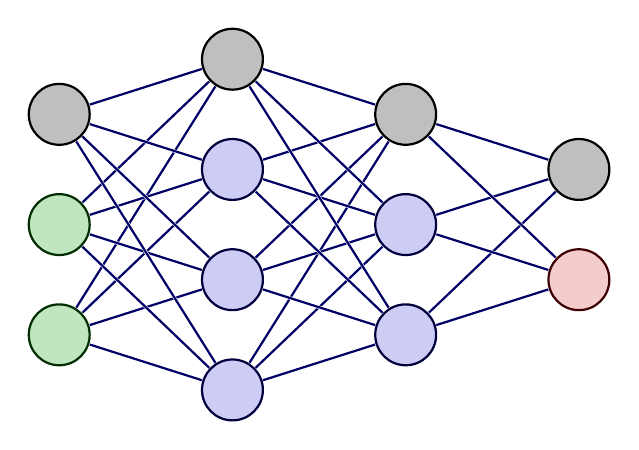
\begin{tikzpicture}[x=2.2cm,y=1.4cm]
        \readlist\Nnod{3,4,3,2} % array of number of nodes per layer

        \foreachitem \N \in \Nnod{ % loop over layers
            \def\curr{\Ncnt} % alias of index of current layer
            \pgfmathsetmacro\prev{int(\Ncnt-1)} % number of previous layer
            \foreach \i [evaluate={\y=\N/2-\i; \x=\curr; \n=\nstyle;}] in {1,...,\N}{ % loop over nodes

                % NODES
                \ifnum\i=1
                    \node[node 0] (N\curr-\i) at (\x,\y) {};
                \else
                    \node[node \n] (N\curr-\i) at (\x,\y) {};
                \fi

                % CONNECTIONS
                \ifnum\curr>1 % connect to previous layer
                    \foreach \j in {1,...,\Nnod[\prev]}{ % loop over nodes in previous layer
                        \draw[connect,white,line width=1.2] (N\prev-\j) -- (N\curr-\i);
                        \draw[connect] (N\prev-\j) -- (N\curr-\i);
                    }
                \fi

            }
        }
    \end{tikzpicture}
    \caption{A small neural network with two hidden layers. The first layer is a Linear layer with 2 input features (plus bias) and 3 output features (plus bias). The second layer is a Linear layer with 3 input features (plus bias) and 2 output features (plus bias). The third layer is a Linear layer with 2 input features (plus bias) and 1 output feature (plus bias). All activation functions are set to the identity.}
    \label{fig:small-nn}
\end{figure}

Let's pick an input $X$ and target $Y$:
\begin{equation*}
    X = \begin{bmatrix}
        1 & 1 & 2 & 2 \\
        2 & 2 & 2 & 3
    \end{bmatrix}, \quad
    Y = \begin{bmatrix}
        1 & 1 & 2 & 2
    \end{bmatrix}
\end{equation*}

This is a small dataset of four samples with two input features and one output feature.

The first step is to prepend the bias feature to the input and to the output:
\begin{equation*}
    A^{[0]} = \tilde{X} = \mqty[
        \color{red} 1 & \color{red} 1 & \color{red} 1 & \color{red} 1 \\
        1 & 1 & 2 & 2 \\
        2 & 2 & 2 & 3
    ], \quad \tilde{Y} = \mqty[
        \color{red} 1 & \color{red} 1 & \color{red} 1 & \color{red} 1 \\
        1 & 1 & 2 & 2
    ]
\end{equation*}

\subsubsection{Forward pass}
\paragraph{Layer 1 (Linear)} The first layer is a Linear layer with 3 input features (plus bias) and 4 output features (plus bias). The weights matrix $W^{[1]}$ is initialized randomly:
\begin{equation*}
    W^{[1]} = \mqty[
        \color{red} 1 & \color{red} 0 & \color{red} 0 \\
        0 & 0 & 1 \\
        0 & 1 & 1 \\
        1 & 0 & 0
    ]
\end{equation*}
\begin{equation*}
    Z^{[1]} = W^{[1]} A^{[0]} = \mqty[
        \color{red} 1 & \color{red} 1 & \color{red} 1 & \color{red} 1 \\
        2 & 3 & 2 & 3 \\
        3 & 4 & 4 & 5 \\
        2 & 2 & 3 & 3
    ]
\end{equation*}

\paragraph{Layer 1 (Activation)} The activation function is applied element-wise, skipping the first row:
\begin{equation*}
    A^{[1]} = \mqty[
        \mqty{\color{red} 1 & \color{red} 1 & \color{red} 1 & \color{red} 1} \\
        g(Z^{[1]}[1\hspace{-0.6ex}:])
    ] = \mqty[
        \color{red} 1 & \color{red} 1 & \color{red} 1 & \color{red} 1 \\
        2 & 3 & 2 & 3 \\
        3 & 4 & 4 & 5 \\
        2 & 2 & 3 & 3
    ]
\end{equation*}

\paragraph{Layer 2 (Linear)} The second layer is a Linear layer with 4 input features (plus bias) and 3 output features (plus bias). The weights matrix $W^{[2]}$ is initialized randomly:
\begin{equation*}
    W^{[2]} = \mqty[
        \color{red} 1 & \color{red} 0 & \color{red} 0 & \color{red} 0\\
        1 & 1 & 0 & 1\\
        -1 & 1 & 2 & -2
    ]
\end{equation*}
\begin{equation*}
    Z^{[2]} = W^{[2]} A^{[1]} = \mqty[
        \color{red} 1 & \color{red} 1 & \color{red} 1 & \color{red} 1 \\
        5 & 6 & 6 & 7 \\
        3 & 6 & 3 & 6
    ]
\end{equation*}

\paragraph{Layer 2 (Activation)} The activation function is applied element-wise, skipping the first row:
\begin{equation*}
    A^{[2]} = \mqty[
        \mqty{\color{red} 1 & \color{red} 1 & \color{red} 1 & \color{red} 1} \\
        g(Z^{[2]}[1\hspace{-0.6ex}:])
    ] = \mqty[
        \color{red} 1 & \color{red} 1 & \color{red} 1 & \color{red} 1 \\
        5 & 6 & 6 & 7 \\
        3 & 6 & 3 & 6
    ]
\end{equation*}

\paragraph{Layer 3 (Linear)} The third layer is a Linear layer with 3 input features (plus bias) and 2 output features (plus bias). The weights matrix $W^{[3]}$ is initialized randomly:
\begin{equation*}
    W^{[3]} = \mqty[
        \color{red} 1 & \color{red} 0 & \color{red} 0 \\
        0 & 1 & -1
    ]
\end{equation*}
\begin{equation*}
    Z^{[3]} = W^{[3]} A^{[2]} = \mqty[
        \color{red} 1 & \color{red} 1 & \color{red} 1 & \color{red} 1 \\
        2 & 0 & 3 & 1
    ]
\end{equation*}

\paragraph{Layer 3 (Activation)} The activation function is applied element-wise, skipping the first row:
\begin{equation*}
    \hat{Y} = A^{[3]} = \mqty[
        \mqty{\color{red} 1 & \color{red} 1 & \color{red} 1 & \color{red} 1} \\
        g(Z^{[3]}[1\hspace{-0.6ex}:])
    ] = \mqty[
        \color{red} 1 & \color{red} 1 & \color{red} 1 & \color{red} 1 \\
        2 & 0 & 3 & 1
    ]
\end{equation*}

Now we compute the loss:
\begin{align*}
    \J(\hat{Y}, \tilde{Y}) &= \frac{1}{m} \sum_{i=1}^{m} \norm{\hat{Y}_i - \tilde{Y}_i}^2\\
    &\;\begin{aligned}
        = \frac{1}{4} \left[\right.&(1 - 1)^2 + (1 - 1)^2 + (1 - 1)^2 + (1 - 1)^2 + \\
        &(2 - 1)^2 + (0 - 1)^2 + (3 - 2)^2 + (1 - 2)^2\left.\right] = 1
    \end{aligned}
\end{align*}

\subsubsection{Backward pass}
To start the backward pass, we need to compute the gradient of the loss \wrt the output of the network:
\begin{equation*}
    \frac{\partial \J}{\partial \hat{Y}} = \frac{2}{m} \left(\hat{Y} - \tilde{Y}\right) = \frac{1}{4} \mqty[
        \color{red} 0 & \color{red} 0 & \color{red} 0 & \color{red} 0 \\
        1 & -1 & 1 & -1
    ] = \pdv{\J}{A^{[3]}}
\end{equation*}
This is now the input of the backward method of the last layer.

\paragraph{Layer 3 (Activation)} The backward method of the Activation layer computes the gradient of the loss \wrt its input $Z^{[3]}$. Since the activation function is the identity, its derivative is 1, and we have:
\begin{equation*}
    \Delta^{[3]} = \pdv{\J}{Z^{[3]}} = \pdv{\J}{A^{[3]}} \odot \mqty[
        \mqty{\color{red} 0 & \color{red} 0 & \color{red} 0 & \color{red} 0} \\
        g'(Z^{[3]}[1\hspace{-0.6ex}:])
    ] = \frac{1}{4} \mqty[
        \color{red} 0 & \color{red} 0 & \color{red} 0 & \color{red} 0 \\
        1 & -1 & 1 & -1
    ]
\end{equation*}

\paragraph{Layer 3 (Linear)} The backward method of the Linear layer computes the gradient of the loss \wrt its weights $W^{[3]}$ and its input $A^{[2]}$:
\begin{gather*}
    \pdv{\J}{W^{[3]}} = \Delta^{[3]} A^{[2]T} = \frac{1}{4} \mqty[
        \color{red} 0 & \color{red} 0 & \color{red} 0 \\
        0 & -2 & -6
    ]\\
    \pdv{\J}{A^{[2]}} = W^{[3]T} \Delta^{[3]} = \frac{1}{4} \mqty[
        \color{red} 0 & \color{red} 0 & \color{red} 0 & \color{red} 0 \\
        1 & -1 & 1 & -1 \\
        -1 & 1 & -1 & 1
    ]
\end{gather*}

\paragraph{Layer 2 (Activation)} The backward method of the Activation layer computes the gradient of the loss \wrt its input $Z^{[2]}$. Since the activation function is the identity, its derivative is 1, and we have:
\begin{equation*}
    \Delta^{[2]} = \pdv{\J}{Z^{[2]}} = \pdv{\J}{A^{[2]}} \odot \mqty[
        \mqty{\color{red} 0 & \color{red} 0 & \color{red} 0 & \color{red} 0} \\
        g'(Z^{[2]}[1\hspace{-0.6ex}:])
    ] = \frac{1}{4} \mqty[
        \color{red} 0 & \color{red} 0 & \color{red} 0 & \color{red} 0 \\
        1 & -1 & 1 & -1 \\
        -1 & 1 & -1 & 1
    ]
\end{equation*}

\paragraph{Layer 2 (Linear)} The backward method of the Linear layer computes the gradient of the loss \wrt its weights $W^{[2]}$ and its input $A^{[1]}$:
\begin{gather*}
    \pdv{\J}{W^{[2]}} = \Delta^{[2]} A^{[1]T} = \frac{1}{4} \mqty[
        \color{red} 0 & \color{red} 0 & \color{red} 0 & \color{red} 0 \\
        0 & -2 & -2 & 0 \\
        0 & 2 & 2 & 0 \\
    ]\\
    \pdv{\J}{A^{[1]}} = W^{[2]T} \Delta^{[2]} = \frac{1}{4} \mqty[
        \color{red} 2 & \color{red} -2 & \color{red} 2 & \color{red} -2 \\
        0 & 0 & 0 & 0 \\
        -2 & 2 & -2 & 2 \\
        3 & -3 & 3 & -3 \\
    ]
\end{gather*}

\paragraph{Layer 1 (Activation)} The backward method of the Activation layer computes the gradient of the loss \wrt its input $Z^{[1]}$. Since the activation function is the identity, its derivative is 1, and we have:
\begin{equation*}
    \Delta^{[1]} = \pdv{\J}{Z^{[1]}} = \pdv{\J}{A^{[1]}} \odot \mqty[
        \mqty{\color{red} 0 & \color{red} 0 & \color{red} 0 & \color{red} 0} \\
        g'(Z^{[1]}[1\hspace{-0.6ex}:])
    ] = \frac{1}{4} \mqty[
        \color{red} 0 & \color{red} 0 & \color{red} 0 & \color{red} 0 \\
        0 & 0 & 0 & 0 \\
        -2 & 2 & -2 & 2 \\
        3 & -3 & 3 & -3 \\
    ]
\end{equation*}

\paragraph{Layer 1 (Linear)} The backward method of the Linear layer computes the gradient of the loss \wrt its weights $W^{[1]}$ and its input $A^{[0]}$:
\begin{gather*}
    \pdv{\J}{W^{[1]}} = \Delta^{[1]} A^{[0]T} = \frac{1}{4} \mqty[
        \color{red} 0 & \color{red} 0 & \color{red} 0 \\
        0 & 0 & 0 \\
        0 & 0 & 4 \\
        0 & 0 & -6
    ]\\
    \pdv{\J}{A^{[0]}} = W^{[1]T} \Delta^{[1]} = \frac{1}{4} \mqty[
        \color{red} 3 & \color{red} -3 & \color{red} 3 & \color{red} -3 \\
        1 & -1 & 1 & -1 \\
        -2 & 2 & -2 & 2
    ] \quad \text{(unused)}
\end{gather*}

\subsubsection{Weight update}

The weights are updated using gradient descent:
\begin{equation*}
    W^{[l]} \gets W^{[l]} - \eta \pdv{\J}{W^{[l]}} \\
\end{equation*}

Setting the learning rate $\eta = 4$ for simplicity\footnote{This value is way too high to have any chance of yielding an improvement in the predictions in any practical example.}, we have: 
\begin{gather*}
    W^{[3]} \gets \mqty[
        \color{red} 1 & \color{red} 0 & \color{red} 0 \\
        0 & 1 & -1
    ] - \mqty[
        \color{red} 0 & \color{red} 0 & \color{red} 0 \\
        0 & -2 & -6
    ] = \mqty[
        \color{red} 1 & \color{red} 0 & \color{red} 0 \\
        0 & 3 & 5
    ]\\
    W^{[2]} \gets \mqty[
        \color{red} 1 & \color{red} 0 & \color{red} 0 & \color{red} 0\\
        1 & 1 & 0 & 1\\
        -1 & 1 & 2 & -2
    ] - \mqty[
        \color{red} 0 & \color{red} 0 & \color{red} 0 & \color{red} 0 \\
        0 & -2 & -2 & 0 \\
        0 & 2 & 2 & 0 \\
    ] = \mqty[
        \color{red} 1 & \color{red} 0 & \color{red} 0 & \color{red} 0\\
        1 & 3 & 2 & 1\\
        -1 & -1 & 0 & -2
    ]\\
    W^{[1]} \gets \mqty[
        \color{red} 1 & \color{red} 0 & \color{red} 0 \\
        0 & 0 & 1 \\
        0 & 1 & 1 \\
        1 & 0 & 0
    ] - \mqty[
        \color{red} 0 & \color{red} 0 & \color{red} 0 \\
        0 & 0 & 0 \\
        0 & 0 & 4 \\
        0 & 0 & -6
    ] = \mqty[
        \color{red} 1 & \color{red} 0 & \color{red} 0 \\
        0 & 0 & 1 \\
        0 & 1 & -3 \\
        1 & 0 & 6
    ]
\end{gather*}

Now a new cycle of forward pass/backward pass/weight update can begin.

\section{Loss} \label{sec:loss}

The final ingredient in the training of a \acl{NN} is the loss function. This function measures the error between the predicted output of the network and the true target values. The goal of training is to minimize this loss function by adjusting the weights of the network through backpropagation.

Also, as seen in \cref{sec:backprop}, the derivative of the loss \wrt the output of the network is needed to start the backpropagation process. \mfnet implements two of the most important loss functions: \ac{MSE}, used mainly in regression tasks, and \ac{CE}, used in classification tasks.

\subsection{\acl{MSE}}
The \ac{MSE} loss function is defined as:
\begin{equation}
    \J(\hat{Y}, Y) = \frac{1}{m} \sum_{i=1}^{m} \norm{\hat{Y}_i - Y_i}_2^2 = \frac{1}{m} \sum_{i=1}^{m} \sum_{j=1}^{n_\text{feat}} (\hat{Y}_{ij} - Y_{ij})^2
\end{equation}
where $\hat{Y}_i$ is the vector of predicted values for the $i$-th sample, $Y_i$ is the vector of true target values for the $i$-th sample and $m$ is the number of samples. It represents the square modulus of the error vector, averaged over all samples.

The gradient matrix of the loss \wrt the output of the network is given by:
\begin{equation}
    \pdv{\J}{\hat{Y}} = \frac{2}{m} (\hat{Y} - Y)
\end{equation}

\subsection{\acl{CE}}
\acl{CE} is a measure that determines the similarity between two probability distributions. In the context of \aclp{NN}, it is commonly used as a loss function for classification tasks, where the predicted output of the network represents a probability distribution over different classes.

\paragraph{Definition}
The \ac{CE} loss function is defined as:
\begin{equation}
    \J(S, Y) = -\frac{1}{m} \sum_{i=1}^{m} \norm{Y_i \odot \log(S_i)}_1 = -\frac{1}{m} \sum_{i=1}^{m} \sum_{j=1}^{C} Y_{ij} \log(S_{ij})
\end{equation}
where $S_{ij}$ is the predicted probability of the $i$-th sample belonging to class $j$, $Y_{ij}$ is the true probability (1 if the sample belongs to class $j$, 0 otherwise), $m$ is the number of samples, and $C$ is the number of classes.

This formula assumes that the predicted outputs $S$ are a probability distribution (i.e., that $0 \leq S_{ij} \leq 1$ and $\sum_{j=1}^{C} S_{ij} = 1\ \forall i$).

Such a distribution can be obtained by applying the softmax function to the raw output logits $Z_{ij}$ of the network. The softmax function is defined as:
\begin{equation}
    S_{ij} = \frac{e^{Z_{ij}}}{\sum_{k=1}^{C} e^{Z_{ik}}}
\end{equation}

To make sure that the \ac{CE} loss has the appropriate input, a softmax is automatically applied before it. The user must not manually insert a softmax layer before the loss (nor does \mfnet define one).

\paragraph{Gradient} The \mono{CELoss} class is responsible for computing the gradient of the \ac{CE} loss \wrt the input logits. This can be broken down in two steps.

\subparagraph{Softmax Gradient} We start by taking the logarithm of the softmax:
\begin{equation*}
    \log(S_{ij}) = Z_{ij} - \log(\sum_{k=1}^{C} e^{Z_{ik}})
\end{equation*}
and then its derivative:
\begin{equation} \label{eq:softmax_grad}
\begin{split}
    \pdv{\log(S_{ij})}{Z_{lt}} &= \pdv{Z_{ij}}{Z_{lt}} - \pdv{\log(\sum_{k=1}^{C} e^{Z_{ik}})}{Z_{lt}}\\
    &= \delta_{ij,lt} - \frac{1}{\sum_{k=1}^{C} e^{Z_{ik}}} \sum_{k=1}^{C} \pdv{e^{Z_{ik}}}{Z_{lt}}\\
    &= \delta_{ij,lt} - \frac{1}{\sum_{k=1}^{C} e^{Z_{ik}}} \sum_{k=1}^{C} e^{Z_{ik}} \delta_{ik,lt}\\
    &= \delta_{ij,lt} - \frac{e^{Z_{it}}}{\sum_{k=1}^{C} e^{Z_{ik}}} \delta_{il}\\
    &= \delta_{ij,lt} - S_{it} \delta_{il}
\end{split}
\end{equation}

The gradient can now be easily obtained by inverting the relation:
\begin{gather*}
    \pdv{\log(S_{ij})}{Z_{lt}} = \frac{1}{S_{ij}} \pdv{S_{ij}}{Z_{lt}}\nonumber\\
    \pdv{S_{ij}}{Z_{lt}} = S_{ij} \pdv{\log(S_{ij})}{Z_{lt}} = S_{ij} (\delta_{ij,lt} - S_{it} \delta_{il})
\end{gather*}

\subparagraph{\ac{CE} Gradient} We can now differentiate the \ac{CE} \wrt the input logits $Z_{lt}$:
\begin{equation}
\begin{split}
    \pdv{\J}{Z_{lt}} &= -\frac{1}{m} \sum_{i=1}^{m} \sum_{j=1}^{C} Y_{ij} \pdv{\log(S_{ij})}{Z_{lt}}\\
    &\overset{(a)}{=} -\frac{1}{m} \sum_{i=1}^{m} \sum_{j=1}^{C} Y_{ij} \left(\delta_{ij,lt} - S_{it} \delta_{il} \right)\\
    &= -\frac{1}{m} \left( Y_{lt} - \sum_{i=1}^{m} \sum_{j=1}^{C} Y_{ij} S_{it} \delta_{il} \right)\\
    &= -\frac{1}{m} \left( Y_{lt} - S_{lt} \sum_{j=1}^{C} Y_{lj} \right)\\
    &\overset{(b)}{=} -\frac{1}{m} \left( Y_{lt} - S_{lt} \right)\\
    &= \frac{S_{lt} - Y_{lt}}{m}
\end{split}
\end{equation}
where in $(a)$ we used the result from \cref{eq:softmax_grad}, and in $(b)$ we used the fact that $Y_i$ is a one-hot encoded vector.

\paragraph{Implementation details} Since the output logits from the network have the bias row (first row set to all 1s), before doing any calculation in the \mono{CELoss} class we remove this row, both from the logits and from the target labels. For numerical stability, the softmax is actually computed as:
\begin{verbatim}
    e_x = np.exp(logits - np.max(logits, axis=0, keepdims=True))
    softmax_pred = e_x / np.sum(e_to_the_x, axis=0, keepdims=True)
\end{verbatim}

To prevent numerical problems arising from $\log(0)$, we also clip the softmax output to a minimum value of $\num{e-100}$.

The \mono{grad} method of the \mono{CELoss} class prepends a row of zeros to the gradient matrix, to match the shape of the input logits.

% \section{\acl*{NN}, Optimizer and Dataloader} \label{sec:nn-optim-data}
In this section we describe the implementation of more high-level objects that can be built using the building blocks described in the previous sections.

\subsection{\acl*{NN}}
A \acl{NN} is made up of a sequence of layers, each one transforming the input tensor into an output tensor, and each one feeding into the next.

As far as coding is concerned, it is a very simple object, and only defines three methods: forward, backward and a method that yields an iterator on all the layers' parameters. This last method is used by the optimizer when performing the update step.

The forward method simply calls the forward method of each layer in sequence, passing the output of one layer as input to the next one.

The backward method does the opposite: it calls the backward method of each layer in reverse order, passing the gradient of the loss with respect to the input of each layer as input to the previous layer.

\subsection{Optimizer}
The optimizer is responsible for updating the parameters of the \acl{NN} during training.

The most basic optimizer is \ac{GD}, which updates the parameters according to the rule:
\begin{equation}
    W^{[l]} \gets W^{[l]} - \eta \pdv{\J}{W^{[l]}}
\end{equation}
where $\eta$ is the learning rate.

The algorithm in this form suffers from many problems, such as having a big computational overhead and not being able to escape local minima. A more robust version is \ac{SGD}, which updates the parameters using a mini-batch (see \cref{sec:dataloader}) instead of the whole dataset. This introduces some stochastic noise in the updates, which can help the optimizer to better explore the space. It also reduces the size of the gradient matrix that needs to be computed, greatly reducing the computational burden.

\paragraph{Implementation details} When training a full \ac{NN} using ReLUs as activation functions, there was often an overflow problem. To help mitigate this, the \mono{Optimizer} class implements gradient clipping, which prevents the gradients from becoming too large by clipping the norm of the gradient tensor to a maximum value provided by the user.

\subsection{Dataloader} \label{sec:dataloader}
The dataloader is responsible for loading the data in mini-batches and shuffling it at the beginning of each epoch. This is important for \ac{SGD} to work properly, as it helps to reduce the correlation between consecutive mini-batches and improves the convergence of the optimizer.

\paragraph{Implementation details} In addition to creating the mini-batches, the\\\mono{DataLoader} class is also responsible for transforming the data, which is usually stored in a \shape{m}{n_\text{features}} matrix (the design matrix), into a format compatible with the \mfnet library: first, the design matrix is transposed, so that each column represents a data sample and each row represents a feature; then, the bias feature is prepended to the input data as a row of 1s. The same transformations are applied to the target data.

\paragraph{Example}
For a complete step-by-step example of how the learning process works, please refer to \cref{sec:example}.

% \section{Training} \label{sec:training}

The \mono{train.py} module provides three convenience functions for training and evaluating neural networks: \mono{train}, \mono{train\_test\_regression}, and\\\mono{train\_test\_classification}.

\paragraph{Overview}
All functions implement the standard training cycle over epochs:
\begin{enumerate}
    \item iterate over the training set in mini-batches (see \cref{sec:dataloader});
    \item forward pass to obtain predictions;
    \item compute the loss;
    \item backward pass to compute gradients;
    \item optionally clip gradients if a maximum norm is specified (before the optimizer step; see \cref{sec:nn-optim-data});
    \item update parameters with the optimizer.
\end{enumerate}
At the end of each epoch, the loss is averaged over all batches and appended to a history that is returned to the caller.

\paragraph{APIs and returned metrics}
\begin{itemize}
    \item \mono{train}: runs training only and returns the per-epoch training loss history.
    \item \mono{train\_test\_regression}: trains and evaluates on a test set each epoch; returns training loss and test loss histories.
    \item \mono{train\_test\_classification}: as above, plus computes test accuracy each epoch using \mono{accuracy} (see \cref{sec:training-utilities}); returns training loss, test loss, and test accuracy histories.
\end{itemize}
Evaluation runs a forward pass on the test set without parameter updates.

% \section{Training utilities} \label{sec:training-utilities}

The most useful function provided by the \mono{trainutils.py} module is\\\mono{train\_test\_split}. This function takes as input two tensors (input data and target data) and splits them into training and test sets.

Other notable functions include \mono{normalize\_features} and\\\mono{denormalize\_features}, which are used to normalize and denormalize the input features, respectively; \mono{one\_hot\_encode} and \mono{one\_hot\_decode}, which are used to convert categorical labels into one-hot encoded vectors and vice versa; and \mono{accuracy}, which computes the accuracy of predictions for classification tasks, i.e., the number of correct predictions divided by the total number of predictions.



\appendix

\newpage
\section{Step-by-step example of an epoch} \label{sec:example}
To better understand how the bias is handled throughout \mfnet, it's helpful to consider a practical example: we'll walk through a forward/backward cycle of a small network with two hidden layers and all the activation functions set to the identity.

\begin{figure}[h]
    \centering
    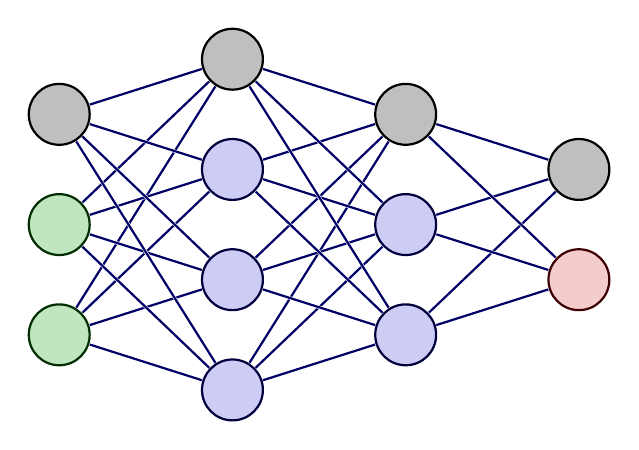
\begin{tikzpicture}[x=2.2cm,y=1.4cm]
        \readlist\Nnod{3,4,3,2} % array of number of nodes per layer

        \foreachitem \N \in \Nnod{ % loop over layers
            \def\curr{\Ncnt} % alias of index of current layer
            \pgfmathsetmacro\prev{int(\Ncnt-1)} % number of previous layer
            \foreach \i [evaluate={\y=\N/2-\i; \x=\curr; \n=\nstyle;}] in {1,...,\N}{ % loop over nodes

                % NODES
                \ifnum\i=1
                    \node[node 0] (N\curr-\i) at (\x,\y) {};
                \else
                    \node[node \n] (N\curr-\i) at (\x,\y) {};
                \fi

                % CONNECTIONS
                \ifnum\curr>1 % connect to previous layer
                    \foreach \j in {1,...,\Nnod[\prev]}{ % loop over nodes in previous layer
                        \draw[connect,white,line width=1.2] (N\prev-\j) -- (N\curr-\i);
                        \draw[connect] (N\prev-\j) -- (N\curr-\i);
                    }
                \fi

            }
        }
    \end{tikzpicture}
    \caption{A small \acl{NN} with two hidden layers. The gray neurons represent the bias features.}
    \label{fig:small-nn}
\end{figure}

Let's pick an input $X$ and target $Y$:
\begin{equation*}
    X = \mqty[
        1 & 2 \\
        1 & 2 \\
        2 & 2 \\
        2 & 3
    ], \quad
    Y = \mqty[1 \\ 1 \\ 2 \\ 2]
\end{equation*}

This is a small dataset of four samples with two input features and one target feature.

First, the \mono{DataLoader} transposes the data and prepends the bias feature:
\begin{equation*}
    A^{[0]} = \tilde{X} = \mqty[
        \color{red} 1 & \color{red} 1 & \color{red} 1 & \color{red} 1 \\
        1 & 1 & 2 & 2 \\
        2 & 2 & 2 & 3
    ], \quad \tilde{Y} = \mqty[
        \color{red} 1 & \color{red} 1 & \color{red} 1 & \color{red} 1 \\
        1 & 1 & 2 & 2
    ]
\end{equation*}

\newpage
\subsection{Forward pass}
Now the \mono{forward} method of the \mono{NeuralNetwork} is called with input data $A^{[0]}$.

\paragraph{Layer 1 (Linear)} The first layer is a Linear layer with 2 input features (plus bias) and 3 output features (plus bias). Suppose the weights matrix $W^{[1]}$ is:
\begin{equation*}
    W^{[1]} = \mqty[
        \color{red} 1 & \color{red} 0 & \color{red} 0 \\
        0 & 0 & 1 \\
        0 & 1 & 1 \\
        1 & 0 & 0
    ]
\end{equation*}

Then, the output of the layer is:
\begin{equation*}
    Z^{[1]} = W^{[1]} A^{[0]} = \mqty[
        \color{red} 1 & \color{red} 1 & \color{red} 1 & \color{red} 1 \\
        2 & 3 & 2 & 3 \\
        3 & 4 & 4 & 5 \\
        2 & 2 & 3 & 3
    ]
\end{equation*}

\paragraph{Layer 1 (Activation)} The activation function is applied element-wise, skipping the first row:
\begin{equation*}
    A^{[1]} = \mqty[
        \mqty{\color{red} 1 & \color{red} 1 & \color{red} 1 & \color{red} 1} \\
        g(Z^{[1]}[1\hspace{-0.6ex}:])
    ] = \mqty[
        \color{red} 1 & \color{red} 1 & \color{red} 1 & \color{red} 1 \\
        2 & 3 & 2 & 3 \\
        3 & 4 & 4 & 5 \\
        2 & 2 & 3 & 3
    ]
\end{equation*}

\paragraph{Layer 2 (Linear)} The second layer is a Linear layer with 3 input features (plus bias) and 2 output features (plus bias). Suppose the weights matrix $W^{[2]}$ is:
\begin{equation*}
    W^{[2]} = \mqty[
        \color{red} 1 & \color{red} 0 & \color{red} 0 & \color{red} 0\\
        1 & 1 & 0 & 1\\
        -1 & 1 & 2 & -2
    ]
\end{equation*}

Then, the output of the layer is:
\begin{equation*}
    Z^{[2]} = W^{[2]} A^{[1]} = \mqty[
        \color{red} 1 & \color{red} 1 & \color{red} 1 & \color{red} 1 \\
        5 & 6 & 6 & 7 \\
        3 & 6 & 3 & 6
    ]
\end{equation*}

\paragraph{Layer 2 (Activation)} The activation function is applied element-wise, skipping the first row:
\begin{equation*}
    A^{[2]} = \mqty[
        \mqty{\color{red} 1 & \color{red} 1 & \color{red} 1 & \color{red} 1} \\
        g(Z^{[2]}[1\hspace{-0.6ex}:])
    ] = \mqty[
        \color{red} 1 & \color{red} 1 & \color{red} 1 & \color{red} 1 \\
        5 & 6 & 6 & 7 \\
        3 & 6 & 3 & 6
    ]
\end{equation*}

\paragraph{Layer 3 (Linear)} The third layer is a Linear layer with 2 input features (plus bias) and 1 output feature (plus bias). Suppose the weights matrix $W^{[3]}$ is:
\begin{equation*}
    W^{[3]} = \mqty[
        \color{red} 1 & \color{red} 0 & \color{red} 0 \\
        0 & 1 & -1
    ]
\end{equation*}

Then, the output of the layer is:
\begin{equation*}
    Z^{[3]} = W^{[3]} A^{[2]} = \mqty[
        \color{red} 1 & \color{red} 1 & \color{red} 1 & \color{red} 1 \\
        2 & 0 & 3 & 1
    ]
\end{equation*}

\paragraph{Layer 3 (Activation)} The activation function is applied element-wise, skipping the first row:
\begin{equation*}
    \hat{Y} = A^{[3]} = \mqty[
        \mqty{\color{red} 1 & \color{red} 1 & \color{red} 1 & \color{red} 1} \\
        g(Z^{[3]}[1\hspace{-0.6ex}:])
    ] = \mqty[
        \color{red} 1 & \color{red} 1 & \color{red} 1 & \color{red} 1 \\
        2 & 0 & 3 & 1
    ]
\end{equation*}

Now we compute the loss, for instance \ac{MSE}:
\begin{align*}
    \J(\hat{Y}, \tilde{Y}) &= \frac{1}{m} \sum_{i=1}^{m} \norm{\hat{Y}_i - \tilde{Y}_i}^2\\
    &\;\begin{aligned}
        = \frac{1}{4} \left[\right.&(1 - 1)^2 + (1 - 1)^2 + (1 - 1)^2 + (1 - 1)^2 + \\
        &+ (2 - 1)^2 + (0 - 1)^2 + (3 - 2)^2 + (1 - 2)^2\left.\right] = 1
    \end{aligned}
\end{align*}

\subsection{Backward pass}
To start the backward pass, we need to compute the gradient of the loss \wrt the output of the network:
\begin{equation*}
    \frac{\partial \J}{\partial \hat{Y}} = \frac{2}{m} \left(\hat{Y} - \tilde{Y}\right) = \frac{1}{4} \mqty[
        \color{red} 0 & \color{red} 0 & \color{red} 0 & \color{red} 0 \\
        1 & -1 & 1 & -1
    ] = \pdv{\J}{A^{[3]}}
\end{equation*}
This is now the input of the \mono{backward} method of the \mono{NeuralNetwork}.

\paragraph{Layer 3 (Activation)} The backward method of the Activation layer computes the gradient of the loss \wrt its input $Z^{[3]}$. Since the activation function is the identity, its derivative is 1, and we have:
\begin{equation*}
    \Delta^{[3]} = \pdv{\J}{Z^{[3]}} = \pdv{\J}{A^{[3]}} \odot \mqty[
        \mqty{\color{red} 0 & \color{red} 0 & \color{red} 0 & \color{red} 0} \\
        g'(Z^{[3]}[1\hspace{-0.6ex}:])
    ] = \frac{1}{4} \mqty[
        \color{red} 0 & \color{red} 0 & \color{red} 0 & \color{red} 0 \\
        1 & -1 & 1 & -1
    ]
\end{equation*}

\paragraph{Layer 3 (Linear)} The backward method of the Linear layer computes the gradient of the loss \wrt its weights $W^{[3]}$ and its input $A^{[2]}$:
\begin{gather*}
    \pdv{\J}{W^{[3]}} = \Delta^{[3]} A^{[2]T} = \frac{1}{4} \mqty[
        \color{red} 0 & \color{red} 0 & \color{red} 0 \\
        0 & -2 & -6
    ]\\
    \pdv{\J}{A^{[2]}} = W^{[3]T} \Delta^{[3]} = \frac{1}{4} \mqty[
        \color{red} 0 & \color{red} 0 & \color{red} 0 & \color{red} 0 \\
        1 & -1 & 1 & -1 \\
        -1 & 1 & -1 & 1
    ]
\end{gather*}

\paragraph{Layer 2 (Activation)} The backward method of the Activation layer computes the gradient of the loss \wrt its input $Z^{[2]}$. Since the activation function is the identity, its derivative is 1, and we have:
\begin{equation*}
    \Delta^{[2]} = \pdv{\J}{Z^{[2]}} = \pdv{\J}{A^{[2]}} \odot \mqty[
        \mqty{\color{red} 0 & \color{red} 0 & \color{red} 0 & \color{red} 0} \\
        g'(Z^{[2]}[1\hspace{-0.6ex}:])
    ] = \frac{1}{4} \mqty[
        \color{red} 0 & \color{red} 0 & \color{red} 0 & \color{red} 0 \\
        1 & -1 & 1 & -1 \\
        -1 & 1 & -1 & 1
    ]
\end{equation*}

\paragraph{Layer 2 (Linear)} The backward method of the Linear layer computes the gradient of the loss \wrt its weights $W^{[2]}$ and its input $A^{[1]}$:
\begin{gather*}
    \pdv{\J}{W^{[2]}} = \Delta^{[2]} A^{[1]T} = \frac{1}{4} \mqty[
        \color{red} 0 & \color{red} 0 & \color{red} 0 & \color{red} 0 \\
        0 & -2 & -2 & 0 \\
        0 & 2 & 2 & 0 \\
    ]\\
    \pdv{\J}{A^{[1]}} = W^{[2]T} \Delta^{[2]} = \frac{1}{4} \mqty[
        \color{red} 2 & \color{red} -2 & \color{red} 2 & \color{red} -2 \\
        0 & 0 & 0 & 0 \\
        -2 & 2 & -2 & 2 \\
        3 & -3 & 3 & -3 \\
    ]
\end{gather*}

\paragraph{Layer 1 (Activation)} The backward method of the Activation layer computes the gradient of the loss \wrt its input $Z^{[1]}$. Since the activation function is the identity, its derivative is 1, and we have:
\begin{equation*}
    \Delta^{[1]} = \pdv{\J}{Z^{[1]}} = \pdv{\J}{A^{[1]}} \odot \mqty[
        \mqty{\color{red} 0 & \color{red} 0 & \color{red} 0 & \color{red} 0} \\
        g'(Z^{[1]}[1\hspace{-0.6ex}:])
    ] = \frac{1}{4} \mqty[
        \color{red} 0 & \color{red} 0 & \color{red} 0 & \color{red} 0 \\
        0 & 0 & 0 & 0 \\
        -2 & 2 & -2 & 2 \\
        3 & -3 & 3 & -3 \\
    ]
\end{equation*}

\paragraph{Layer 1 (Linear)} The backward method of the Linear layer computes the gradient of the loss \wrt its weights $W^{[1]}$ and its input $A^{[0]}$:
\begin{gather*}
    \pdv{\J}{W^{[1]}} = \Delta^{[1]} A^{[0]T} = \frac{1}{4} \mqty[
        \color{red} 0 & \color{red} 0 & \color{red} 0 \\
        0 & 0 & 0 \\
        0 & 0 & 4 \\
        0 & 0 & -6
    ]\\
    \pdv{\J}{A^{[0]}} = W^{[1]T} \Delta^{[1]} = \frac{1}{4} \mqty[
        \color{red} 3 & \color{red} -3 & \color{red} 3 & \color{red} -3 \\
        1 & -1 & 1 & -1 \\
        -2 & 2 & -2 & 2
    ] \quad \text{(unused)}
\end{gather*}

\subsection{Weight update}

The weights are updated using the \ac{SGD} optimizer:
\begin{equation*}
    W^{[l]} \gets W^{[l]} - \eta \pdv{\J}{W^{[l]}} \\
\end{equation*}

Setting the learning rate $\eta = 4$ for simplicity\footnote{This value is way too high to have any chance of yielding an improvement in the predictions in any practical example.}, we have: 
\begin{gather*}
    W^{[3]} \gets \mqty[
        \color{red} 1 & \color{red} 0 & \color{red} 0 \\
        0 & 1 & -1
    ] - \mqty[
        \color{red} 0 & \color{red} 0 & \color{red} 0 \\
        0 & -2 & -6
    ] = \mqty[
        \color{red} 1 & \color{red} 0 & \color{red} 0 \\
        0 & 3 & 5
    ]\\
    W^{[2]} \gets \mqty[
        \color{red} 1 & \color{red} 0 & \color{red} 0 & \color{red} 0\\
        1 & 1 & 0 & 1\\
        -1 & 1 & 2 & -2
    ] - \mqty[
        \color{red} 0 & \color{red} 0 & \color{red} 0 & \color{red} 0 \\
        0 & -2 & -2 & 0 \\
        0 & 2 & 2 & 0 \\
    ] = \mqty[
        \color{red} 1 & \color{red} 0 & \color{red} 0 & \color{red} 0\\
        1 & 3 & 2 & 1\\
        -1 & -1 & 0 & -2
    ]\\
    W^{[1]} \gets \mqty[
        \color{red} 1 & \color{red} 0 & \color{red} 0 \\
        0 & 0 & 1 \\
        0 & 1 & 1 \\
        1 & 0 & 0
    ] - \mqty[
        \color{red} 0 & \color{red} 0 & \color{red} 0 \\
        0 & 0 & 0 \\
        0 & 0 & 4 \\
        0 & 0 & -6
    ] = \mqty[
        \color{red} 1 & \color{red} 0 & \color{red} 0 \\
        0 & 0 & 1 \\
        0 & 1 & -3 \\
        1 & 0 & 6
    ]
\end{gather*}

Now a new cycle of forward pass/backward pass/weight update can begin.


\end{document}

% Part 1: mfnet implementation
% \begin{enumerate}
%     \item information flow in a NN
%     \item basic data structure: Tensor
%     \item layer: Linear and Activations
%     \item Backprop
%     \item losses: MSE an CE
%     \item nn, optimizer
%     \item train helper function
%     \item trainutils?
% \end{enumerate}

% Part 2: comparison with pytorch
% \begin{enumerate}
%     \item Regression task
%     \item Classification task
% \end{enumerate}
